\section{Image Processing}
% Readily compressed and reduced data containing a few relevant spectral signatures across geo-referenced coordinates may efficiently be transmitted to ground enabling faster operational response to investigate target(s) in-situ.
\textcolor{blue}{Contribution(4): "To reduce the large hyperspectral data size to improve latency between space segment and end user as well as to save onboard power and provide high accuracy and resolution in the data to make the concept feasible, a carefully designed image processing pipeline is presented with algorithm elements that are implemented both on ground and on-board HYPSO-1. Key objectives are to perform compression, image registration, geo-referencing, super-resolution, classification and target detection on the hyperspectral data." Key points to keep in mind while writing this section are:
\begin{itemize}
\item Present an overview of the required/planned image processing pipeline.
    \item How does compression (CCSDS123v1 and Dimensionality Reduction) \emph{enable} and improve the CONOPS described in section \ref{sec:mission-design}?
    \item How does the image processing pipeline enable accurate data "geometrically" (image registration) and radiometrically (atmos. correction, smile/keystone, calibration)?
    \item How does the image processing pipeline guarantee $<100$ m resolution, RE: section \ref{sec:mission-design}, in the image pixels given the strategy discussed in section \ref{sec:sampling}?
    \item How does the image processing pipeline enable detection of relatively faint optical signatures, e.g. algal blooms - the mission objective?
    \item How does the image processing pipeline enable interpretable data (geo-referencing, classification)?
    \item How does the image processing pipeline handle atmospheric correction?
    \item How do the data and power budget requirements determine the onboard image processing pipeline (especially compression and DR), will it be feasible and is it implementable?
\end{itemize}}
% The HYPSO satellite will process the collected data on board the satellite before downlinking it. 
% \subsection{Why on-board image processing}

The constraint on the HYPSO-1 mission that mandates an on-board image processing pipeline is its limited data downlink budget and power budget. 

Considering that HYPSO will have a radio link to the ground station for just over 6 minutes on an average pass, the full data cube would take over 100 orbits to downlink, or about 7 days, which is longer than HYPSO's real-time data access requirement permits. 
HYPSO-1 includes on-board image processing to reduce the size of the data to downlink, while retaining as much useful information as possible. The on-board image processing as a whole will thus be oriented towards either reducing the size of the total data set or towards extracting useful information into a smaller data package. 
In reducing the size of the data packages, the image processing pipeline will also enable HYPSO-1 to study the dynamics of an oceanographic phenomena, by permitting the same location to be imaged multiple times in a day. 
\subsection{Desired data products}

The HYPSO satellite will produce data both for further analysis on the ground and for interfacing with in-situ agents. 
The dual purposes of the HYPSO data leads to multiple data format definitions: (A) the standard format consists of a compressed datacube which will be analyzed further on the ground and (B) the operational format which consists of directly actionable data that can be used to inform the actions of in-situ agents or for monitoring algal blooms without the need to manually process the data through an intermediate stage. 
The operational data format is flexible: it can consist of chlorophyll estimates, a classification map, a probability heatmap, or other data formats defined during the mission. 
Then, the operational data format listed in table \ref{tab:data-types} which lists the data size after dimensionality reduction to 20 bands, can be thought of as an upper bound on the size of the operation data.

% https://app.diagrams.net/#G1VghNiGzg5It9wcmylNQLFkDfrnwN8lq1

\begin{figure*}
    \centering
    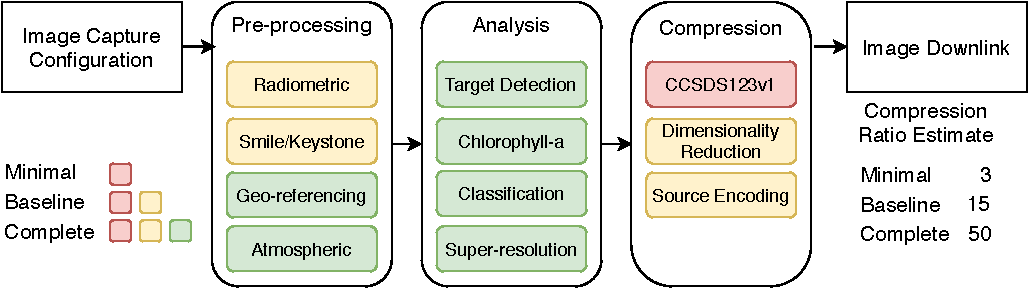
\includegraphics[width = 0.9\textwidth]{figs/img_processing/pipeline_figure_concept_paper.pdf}
    \caption{Illustration of proposed imaging pipelines. Minimal for launch, baseline for the first updates, and complete when reached maturity.}
    \label{fig:image-processing-pipelines}
\end{figure*}

\subsection{Image processing architecture}

A modular image processing pipeline enables HYPSO to downlink the minimal data product, while also permitting the satellite to downlink highly processed and reduced but relevant data (figure \ref{fig:image-processing-pipelines}).
Modules can be interchanged to create new operational data products.
Moreover, different hardware can be utilized for different components of the pipeline. 
For example, compression algorithms, based on the CCSDS123v1 standard, have been developed to run on both the CPU and the FPGA \cite{Fjeldtvedt2018}. 
While the FPGA implementation is faster, the CPU implementation allows for lossy compression, which can increase the data throughput. 
The modular design thus allows the operators to switch between the modules as needed (and the module processing configuration will be stored in the metadata for a particular image). 
However, several specific orderings of the modules are designated as target pipelines in order to maintain constistency among the data products.
Note that $12\times$ binning is incorporated into the image acquisition itself, so the most raw data is reduced before the image processing pipelines begin.
Three of the target pipelines are discussed below. 

% The planned on-board processing is divided into multiple different pipelines, illustrated in figure \ref{fig:image-processing-pipelines}, that share a basic structure, i.e. some level of processing has to be performed regardless, while others may only improve the timeliness of desired data products or reduce the expected data volume to be down-linked. In the subsequent section a high-level description of the software used and planned in the on-board processing is provided.
% \subsubsection{Settings \& Pre-processing}
% The HSI camera will collect spectrograms at a rate of 15-40 Hz. 
% The data rate is limited by the GigE that connects the camera to the breakout board, but by reducing the area of interest or doing sub-sampling in the spectral dimension, the rate at which frames are collected is adjusted \cite{varntresk2019assembly}. 
% It is expected that the imaging sensor of the HSI camera will have some distortions as a result of the optics, and that the sensitivity of given pixels will change over time. 
% Pre-processing, the initial stage of the imaging pipeline seeks to accommodate these undesirable artifacts.

\begin{table*}[htbp]
	\caption{Uncompressed Data Products*}
	\label{tab:data-products}
	\centering
	\begin{tabular}{l | r r r r}
	\hline
	& bands & pixel size (bits) & signatures (MB) & total (MB) \\
	\hline
	Raw & 1200 & $16$& - &984\hspace{10 pt} \hspace{1 pt} \\
	Binned & 100 & $16$ & - & 82.0\hspace{4 pt} \hspace{1 pt} \\
	Dim. reduced & 20 & $16$ & - & 16.4\hspace{4 pt} \hspace{1 pt} \\
	Classification (16 classes) & 1 & $4$ & 0.003 & 0.41 \hspace{1 pt} \\
	Classification (256 classes) & 1 & $8$ & 0.051 & 0.88 \hspace{1 pt} \\
	Target detection (only ACE) & 1 & $16$ & - & 0.82 \hspace{1 pt} \\
	Target detection (with abundance) & 2 & $16$ & - & 1.64 \hspace{1 pt} \\
	Target coordinates (top 100) & n/a & $16$ & - & 0.001 \\
	\hline
	\end{tabular}
	
	\begin{tabular}{c}
		*assuming 1139$\times$720 spatial pixels. \hl{what about spatial compression - jpeg?}
	\end{tabular}
	\vspace*{-\baselineskip}

\end{table*}

\subsubsection{Minimal on-board image processing}
\hl{Joe, Sivert \\}
The minimal on-board image processing pipeline (MOBIP) configuration of the image processing pipeline will typically reduce the size of the data by a factor of 2.5 or more and demonstrate the capability of on-board image processing. 
It consists of image acquisition, compression, and downlinking of the data. 
The compression is implemented on the FPGA of the OPU \cite{Fjeldtvedt2018, orlandic_parallel_2019}. 
Although it is simple, this pipeline forms the basis for all the others. 

\subsubsection{Baseline on-board image processing pipeline}
\hl{Joe, Sivert \\}
The baseline on-board image processing pipeline (BOBIP) configuration adds two important components to MOBIP, before lossless compression. The first of these is a smile and keystone correction, which adjusts the data to account for systematic measurement errors inherent to the imager \cite{Henriksen2019}. 
The second of these is dimensionality reduction, which allows for control of the size of the data package while retaining most of the information of the image. 
The smile and keystone correction is applied before the dimensionality reduction to prevent the dimensionality reduction from modeling systematic, but reversible artifacts from becoming irrevocably intertwined with the data. 

The On-the-Fly-Processing (OTFP) algorithm can be used as dimensionality reduction in order to summarize the spectral information with minimal loss of useful systematic information while simultaneously improving SNR \cite{Vit17}. 
The size of the data package can be controlled by adjusting the number of OTFP bands which are downlinked. 
Thus smile and keystone correction precedes it to avoid imprinting systematic artifacts into the reduced data. 
The residuals from the dimensionality reduction can be down-linked and analysed to provide insight as to what kind of information is being reduced away \cite{Vit17}.
Once it is tested, the BOBIP pipeline will become the standard data format. 
Moreover, dimensionality reduction will increase the speed of modules placed after it in a pipeline because there will be fewer bands to process \cite{Bakken2019SPIE}. 

\subsubsection{Target detection on-board image processing pipeline}
\hl{Joe, Sivert \\}
Another way to expand MOBIP is to add a target detection (TD) module before compression. 
Hyperspectral data is amenable to target detection because of its numerous imaging channels.
By incorporating spectral information about the background scene, TD algorithms can locate sub-pixel spectral signatures. 
The 2D heat maps produced by TD are small enough to downlink data quickly (table \ref{tab:data-types}), and can be immediately used to guide in-situ agents without requiring additional processing on the ground. \hl{Make explicit in Table IV}

The Adaptive Cosine Estimator (ACE) is a target detection algorithm in hyperspectral data that is often used to determine how likely it is that a pixel contains a particular spectral signature \cite{Manolakis2002, Manolakis2005}.
Both software and software-hardware co-design versions of the algorithm have been developed for OPU. 
Acceleration on the FPGA results in a speedup factor of about 28$\times$ relative to software implementations \cite{dijehw19_meco}. 
Effective use of ACE requires spectral knowledge about the targets to be observed. 
A spectrum can either be estimated from data in the lab, which is susceptible to calibration inconsistencies between the lab camera and the satellite camera, or it can be estimated directly from the satellite data, so that the target spectrum and input data are subject to the same limitations. 
A complementary algorithm, the fraction estimator, complements ACE by determining how much of a target is in a given pixel, which leads to the 2 bands seen in table \ref{tab:data-products}. 

\subsection{Developing advanced on-board image processing pipelines}

Some algorithms are still in development, and depending on the end-user that a given pass is targeting, different data products will be desirable.
As part of the reconfigurability of OPU, these future processing pipelines could become a part of the on-going mission. 
These algorithms include image registration, geo-referencing, atmospheric corrections, super-resolution, and classification. 
Several of these kinds of algorithms utilize the RGB camera in addition to the HSI, so it must be drawn into the image processing pipelines. 

Super-resolution algorithms are being adapted to enhance the spatial resolution of remotely sensed images \cite{Park2003, Garrett2019} and to provide improved detectability of features of interest in turn. \hl{this should be emphasized and written about further - crucial for slew maneuver and the core of this paper}
%The latter may give more accurate classification and target detection with fine spatial resolution and high spectral resolution in the image \cite{Manolakis2002, Manolakis2005, Bakken2019SPIE}.


\subsubsection{Upload/reprogram Capability (TENTATIVE)}
\hl{Joe, Sivert \\}
Both the software and FPGA configurations are planned to be updated during the operation of the satellite \cite{Gjersund2020}. First, the software update must be stringently tested on the ground, both in terms of timelinesss and resource usage. Then it must be uplinked to the satellite, which can take several passes. The payload will retain a \textit{golden image}, a version of the operating system and software known to have worked, that it will revert to in case of an update failure. 

\subsubsection{Ground Processing Pipeline}
\hl{Joe, Sivert \\}
An additional image processing pipeline should operate on the ground to (1) prepare data for end users, (2) assist in calibrating the camera in-flight, and (3) to test algorithms before uploading them to the satellite for on-board image processing. 
Some of the components of the pipeline such as geo-referencing and super-resolution are also amenable to being applied to the data after downlinking because they either require access to refence libraries or are computationally intensive.























% \hl{I'm rewriting everything that comes after this - J}

% Readily compressed and reduced data containing the relevant information across geo-referenced coordinates may efficiently be transmitted to ground enabling faster operational response to investigate target(s) of interest in-situ.

% CCSDS123 compression techniques on Field-Programmable-Gate-Array (FPGA) have proven useful for real-time processing and relatively fast lossless data-reduction of large hyperspectral data \cite{Fjeldtvedt2018}.



% \begin{table*}[]
% \begin{tabular}{lllll}
% \textbf{Method}           & \textbf{Purpose} & \textbf{Pipeline} & \textbf{Description}                                      & \textbf{Compression Factor} \\ \hline
% Radiometric Calibration   & Pre-processing   & Baseline          & Ensure correct radiometric intensities in the spectograms & N/A                         \\
% Smile/Keystone Correction & Pre-processing   & Baseline          & Correct for smile and keystone in the spectrograms        & N/A                         \\
% Atmospheric Correction    & Pre-processing   & Complete          & Correct for atmospheric effect on transmitted spectra     & N/A                         \\
% Geo-Refrencing            & Pre-processing   & Compelete         & Correlate each pixel with a location                      & N/A                         \\
% Dimensionality Reduction  & Pre-processing   & Baseline          & Denoising of image cube, data reduction                   & num\_spectra/num\_loadings  \\
% Super-Resolution          & Analysis         & Complete          & Increase spatial resolution of aquired image cube         & TBD                         \\
% Target Detection          & Analysis         & Complete          & Probability map of target                                 & num\_spectra/num\_targets   \\
% Chlorophyll-a             & Analysis         & Complete          & Estimate the chl-a content in an area                     & num\_spectra                \\
% Classification            & Analysis         & Complete          & Divide the data into spectrally distinct classes          & num\_spectra/num\_classes   \\
% CCSDS123v1                & Compression      & Minimal           & Lossless compression of image cube                        & $\sim$3                     \\
% Dimensionality Reduction  & Compression      & Baseline          & Lossy compression of image cube                           & num\_spectra/num\_loadings  \\
% Source Encoding           & Compression      & Baseline          & Lossless compression of data for transmission             & TBD                        
% \end{tabular}
% \end{table*}






